% *======================================================================*
%  Cactus Thorn template for ThornGuide documentation
%  Author: Ian Kelley
%  Date: Sun Jun 02, 2002
%  $Header$                                                             
%
%  Thorn documentation in the latex file doc/documentation.tex 
%  will be included in ThornGuides built with the Cactus make system.
%  The scripts employed by the make system automatically include 
%  pages about variables, parameters and scheduling parsed from the 
%  relevent thorn CCL files.
%  
%  This template contains guidelines which help to assure that your     
%  documentation will be correctly added to ThornGuides. More 
%  information is available in the Cactus UsersGuide.
%                                                    
%  Guidelines:
%   - Do not change anything before the line
%       % BEGIN CACTUS THORNGUIDE",
%     except for filling in the title, author, date etc. fields.
%   - You can define your own macros are OK, but they must appear after
%     the BEGIN CACTUS THORNGUIDE line, and do not redefine standard 
%     latex commands.
%   - To avoid name clashes with other thorns, 'labels', 'citations', 
%     'references', and 'image' names should conform to the following 
%     convention:          
%       ARRANGEMENT_THORN_LABEL
%     For example, an image wave.eps in the arrangement CactusWave and 
%     thorn WaveToyC should be renamed to CactusWave_WaveToyC_wave.eps
%   - Graphics should only be included using the graphix package. 
%     More specifically, with the "includegraphics" command. Do
%     not specify any graphic file extensions in your .tex file. This 
%     will allow us (later) to create a PDF version of the ThornGuide
%     via pdflatex. |
%   - References should be included with the latex "bibitem" command.  
%   - For the benefit of our Perl scripts, and for future extensions, 
%     please use simple latex.     
%
% *======================================================================* 
% 
% Example of including a graphic image:
%    \begin{figure}[ht]
%       \begin{center}
%          \includegraphics[width=6cm]{MyArrangement_MyThorn_MyFigure}
%       \end{center}
%       \caption{Illustration of this and that}
%       \label{MyArrangement_MyThorn_MyLabel}
%    \end{figure}
%
% Example of using a label:
%   \label{MyArrangement_MyThorn_MyLabel}
%
% Example of a citation:
%    \cite{MyArrangement_MyThorn_Author99}
%
% Example of including a reference
%   \bibitem{MyArrangement_MyThorn_Author99}
%   {J. Author, {\em The Title of the Book, Journal, or periodical}, 1 (1999), 
%   1--16. {\tt http://www.nowhere.com/}}
%
% *======================================================================* 

% If you are using CVS use this line to give version information
% $Header$

\documentclass{article}

% Use the Cactus ThornGuide style file
% (Automatically used from Cactus distribution, if you have a 
%  thorn without the Cactus Flesh download this from the Cactus
%  homepage at www.cactuscode.org)
\usepackage{../../../../doc/latex/cactus}

\begin{document}

% The author of the documentation
\author{Miguel Alcubierre/Latex version by Peter Diener} 

% The title of the document (not necessarily the name of the Thorn)
\title{AHFinder}

% the date your document was last changed, if your document is in CVS, 
% please us:
%    \date{$ $Date$ $}
\date{$ $Date$ $}

\maketitle

% Do not delete next line
% START CACTUS THORNGUIDE

% Add all definitions used in this documentation here 
%   \def\mydef etc

% Add an abstract for this thorn's documentation
\begin{abstract}
Finding Apparent Horizons in a numerical spacetime
\end{abstract}

% The following sections are suggestive only.
% Remove them or add your own.

\section{Purpose}

Thorn {\tt AHFinder} finds Apparent Horizons (AHs) in numerical
spacetimes. It calulates various quantities like horizon area and
its corresponding mass.

\section{Using AHFinder}

Thorn AHFinder can be used either with a minimization or a flow algorithm.
\subsection{Parameters}
\subsubsection*{General parameters}
\begin{itemize}
\item {\tt ahfinder::ahf\_active} (steerable) \\
        To activate the thorn set ahf\_active = "yes". This parameter is set
        by default to "no". \\
\item {\tt ahfinder::ahf\_flow} (steerable) \\
        By default the minimization algorithm is used. To switch to the
        flow algorithm one has to set ahf\_flow = "yes"
\end{itemize}
\subsubsection*{Parameters used in evolutions}
\begin{itemize}
\item {\tt ahfinder::ahf\_findevery} (steerable) \\
        Specifies how often the finder is called. The default is to find
        horizons at every iteration.
\item {\tt ahfinder::ahf\_findafter} (steerable) \\
        The number of iterations after which the thorn is called the
        first time can be specified by this parameter. Here the default is 0,
        calling the thorn also on the initial time slice.
\item {\tt ahfinder::ahf\_findaftertime} \\
        Instead of specifying the number of iterations, one can specify
        after how much coordinate time the thorn is called the first time.
        When different from zero, this parameter overrides the value of
        ahf\_findafter. Default here is also 0.
\end{itemize}
\subsubsection*{Parameters specifying the expansion of the surface in sperical
                harmonics.}
\begin{itemize}
\item {\tt ahfinder::ahf\_lmax} \\
        The maximal number of terms in the expansion in $\theta$. The default
        value is 8. The maximal value is 19.
\item {\tt ahfinder::ahf\_phi} (steerable) \\
        If axisymmetry is expected the surface does not need to be
        expanded in phi. This is the default. To look for non-axisymmetric
        surface use ahf\_phi = "yes".
\item {\tt ahfinder::ahf\_[xyz]c} (steerable) \\
        Sets the x-, y-, and z-coordinates of the center of the expansion.
        The default is the origin (ahf\_xc = 0, ahf\_yc = 0, ahf\_zc = 0).
        The center of the expansion should be set inside the expected
        apparent horizon, otherwise the algorithm will fail.
\item {\tt ahfinder::ahf\_wander} \\
        The center of the expansion can also be allowed to move. To do this
        use ahf\_wander = "yes". However, this only works with the
        minimization algorithm. The default is for the center not to move.
\item {\tt ahfinder::ahf\_r0} (steerable) \\
        Sets the radius of the initial sphere. The default is 0.0, forcing
        the largest sphere possible in the grid.
\end{itemize}
\subsubsection*{Looking for three horizons}
The finder can also be used to look for three horizons each time.
This is done by just running the algorithm three consecutive times
with different initial guesses, and is useful for simulations of
black hole collisions.
\begin{itemize}
\item {\tt ahfinder::ahf\_find3} \\
        Set ahf\_find3 = "yes" to search for three horizons. The default is
        to look for only one horizon.
\item {\tt ahfinder::ahf\_[xyz]\_[012]} (steerable) \\
       Sets the x-, y-, and z-coordinates of the center of the expansion for
       horizon 0, 1 and 2. The default in each case is the origin.
\item {\tt ahfinder::ahf\_r0\_[0-2]} (steerable) \\
        Sets the radius of the initial spheres for horizon 0, 1 and 2.
        The default in all cases is 0.0, forcing the largest sphere possible
        in the grid.
\end{itemize}
\subsubsection*{Further parameters for the initial guess}
The initial guess can be furthermore controlled by some parameters
which are set to "no" by default.
\begin{itemize}
\item {\tt ahfinder::ahf\_guessold} (steerable) \\
        To use on old horizon as initial guess set ahf\_guessold = "yes".
        However, if during the evolution the apparent horizon jumps
        discontinuously it might be lost by using this option.
\item {\tt ahfinder::ahf\_nn0, ahfinder::ahf\_nn2} \\
        If no old horizon is used the inital guess can be specified
        further for the minimization algorithm. This algorithm is
        sensitive to the initial guess, so this is important. The initial
        guess is set up by an expansion in spherical harmonics in the
        first two coefficients (l=0,l=2). The default for both these
        parameters are 10, in which case the algorithm tests 100 different
        combinations to find the best initial guess.
\item {\tt ahfinder::ahf\_sloppyguess} \\
        It is also possible to use only a sphere as initial guess. This
        is much faster and is done by using ahf\_sloppyguess = "yes". In this
        case a number of spheres (specified by ahf\_nn0) with different radii
        are tested for the initial guess.
\item {\tt ahfinder::ahf\_inner} \\
        If one wants to look for an inner horizon instead of an outer
        one, use ahfinder::ahf\_inner = "yes". This only works with the
        minimization algorithm.
\end{itemize}
\subsubsection*{Parameters for surface intergrals}
\begin{itemize}
\item {\tt ahfinder::ahf\_ntheta} (steerable) \\
        The number of subdivisions in $\theta$. Default is 200.
\item {\tt ahfinder::ahf\_nphi} (steerable) \\
        The number of subdivisions in $\phi$. Default is 200.
\end{itemize}
\subsubsection*{Parameters indicating symmetries}
\begin{itemize}
\item {\tt ahfinder::ahf\_ref[xyz]} (steerable) \\
        Specifies the existence of reflection symmetry on the yz-plane,
        xz-plane and xy-plane respectively. By default all are set to "no".
\item {\tt ahfinder::ahf\_octant} (steerable) \\
        Octant symmetry is specified by using ahf\_octant = "yes". This is set
        to "no" by default. Possible parmeter settings are "yes" for reflection
        symmetries on all three coordinate planes and "high" for an additional
        rotational symmetry of $\pi/2$ around the z axis.
\item {\tt ahfinder::ahf\_cartoon} (steerable) \\
        A further symmetry can (must) be specified when running with the
        "axisymmetric" mode given by the Cartoon method by using
        ahf\_cartoon = "yes". This is set to "no" by default.
\end{itemize}
\subsubsection*{Parameters for minimization algorithm}
\begin{itemize}
\item {\tt ahfinder::ahf\_tol} \\
        Sets the tolerance for the minimization algorithm. The default
        value is 0.1.
\item {\tt ahfinder::ahf\_maxiter} \\
        Sets the maximum number if iterations for each step of the POWELL
        algorithm. The default value is 10.
\item {\tt ahfinder::ahf\_minarea} \\
        Usually the square of the expansion is minimized. To switch to
        minimization of the area one can use ahf\_minarea = "yes"
        (default is "no"). Notice that only for time symmetric data the
        surface found by area minimization will correspond to an apparent
        horizon.
\end{itemize}
\subsubsection*{Parameters for the flow algorithm}
\begin{itemize}
\item {\tt ahfinder::ahf\_flow} (steerable) \\
        The fow algotithm is used by setting ahf\_flow = "yes". The default
        is "no"
\item {\tt ahfinder::ahf\_flowiter} (steerable) \\
        Sets the maximum number of iterations for the flow algorithm. The
        default value is 200.
\item {\tt ahfinder::ahf\_flowtol} \\
        Sets the tolerance for the flow. The default value is 0.0001.
\item {\tt ahfinder::ahf\_flowa} \\
        Sets the $\alpha$ parameter for the flow. The default value is 0.01.
\item {\tt ahfinder::ahf\_flowb} \\
        Sets the $\beta$ parameter for the flow. The default value is 0.5.
\item {\tt ahfinder::ahf\_flowh} \\
        Sets the weight of $H$ flow. The default value is 0.0.
\item {\tt ahfinder::ahf\_flowc} \\
        Sets the weight of $C$ flow. The default value is 1.0.
\item {\tt ahfinder::ahf\_flown} \\
        Sets the weight of $N$ flow (not yet implemented). The default
        value is 0.0.
\end{itemize}
The character of the different flows and the $\alpha$ and $\beta$
parameters are described in Carsten Gundlach's paper on his
pseudo-spectral apparent horizon finder (gr-qc/9707050).
\subsubsection*{Parameters for output}
\begin{itemize}
\item {\tt ahfinder::ahf\_logfile} \\
        By default no logfile for AHFinder is written. To obtain a log
        file one must set ahf\_logfile = "yes".
\item {\tt ahfinder::ahf\_verbose} \\
        if ahf\_verbose = "yes" messages are printed to screen at the
        beginning and the end of the algorithm. This is the default.
\item {\tt ahfinder::ahf\_veryverbose} \\
        if ahf\_veryverbose = "yes" messages are also printed to screen
        during the iteration process. The default is "no".
\item {\tt ahfinder::ahf\_2Doutput} (steerable) \\
        To get 2D output of grid functions use ahf\_2Doutput = "yes" (default
        is "no"). The output is controlled be the thorn itself, not by cactus
        standard output.
\item {\tt ahfinder::ahf\_3Doutput} (steerable) \\
        In future versions to get 3D output of grid functions use
        ahf\_3Doutput = "yes" (default is "no").
\item {\tt ahfinder::ahf\_areamap} \\
        To get an area map use ahf\_areamap = "yes" (default is "no").
        This is useful for looking at the behaviour of the area for
        surfaces close to the horizon.
\end{itemize}
\subsubsection*{Parameters for mask}
\begin{itemize}
\item {\tt ahfinder::ahf\_mask} (steerable) \\
        The mask is 0 inside the horizon and 1 outside, and is used in
        black-hole excision techniques. By default the mask is off. It
        can be enabled by setting ahf\_mask = "strong", which sets the mask
        only if the finder is sure that a horizon was found, or by setting
        ahf\_mask = "weak", which makes the finder set the mask also if a
        horizon is probably there but either the resolution or lmax are to
        low to really resolve it.
\item {\tt ahfinder::ahf\_masktype} (steerable) \\
        The mask can be of two types. Either ahf\_masktype = "simple",
        which masks a cube contained inside the horizons, or ahf\_masktype
        = "lego", which masks a lego-sphere.
\item {\tt ahfinder::ahf\_maskshrink} (steerable) \\
        Sets a buffer zone between the region inside the horizon and the
        region where the mask is 0, by limiting the mask to a region smaller
        than ahf\_maskshrink times the horizon radius. The default value
        is 0.8.
\item {\tt ahfinder::ahf\_maskbuffer} (steerable) \\
        Sets a buffer zone between the region inside the horizon and the
        region where the mask is 0 with a width of at least ahf\_maskbuffer
        grid points. The default value is 5.
\end{itemize}
\subsection{Minimal parameter settings}
Usually only a few of the parameters described above are needed in the
parameter file. The simplest parameter settings for using the flow
algorithm for a full 3D horizon with a large sphere as initial guess is
{\tt
\begin{verbatim}
interpolation_order = 2     # Second order interpolation
ahf_active          = "yes"
ahf_flow            = "yes"
ahf_phi             = "yes"
\end{verbatim}
}
This looks for a non-axisymmetric horizon around the origin with lmax = 8
and using the flow algorithm. It starts with the largest sphere that fits
in the 3D grid and outputs 2D grid functions. The other parameters can be
used if needed.
\subsection{Hints for parameter settings}
In full 3D the flow algorithm is faster than the minimization algorithm.
However, in cases when there are very few terms in the expansion in
spherical harmonics the minimization can be faster. In axisymmetry this
typically happens for lmax$\leq 10$.

While the default settings usually work fine, they can be changed to meet
special purposes:
\begin{itemize}
\item If the horizon is expected to be far from spherical the parameter
    ahf\_lmax can be set to a higher value. 12 should be high enough.
    However, only values up to 20 are supported.
\item If the latter parameter is set to a value higher than 8 then the
    parameter ahf\_maxiter can be raised to, e.g., 14. This can be useful
    since more iterations can be necessary for higher coefficients of the
    expansion.
\end{itemize}
\subsection{Output to Files}
The output of the thorn consists of two gridfunctions and several one
dimensional output files.
\begin{itemize}
\item To depict the position of the horizon, the most important files are
    ahfgrid\_2d\_...ieee. These files contain a 2D gridfunction whose zero
    level locates the horizon.
\item The files ahf\_exp\_2d\_...ieee show the expansion of outgoing photons
    on the level set of the gridfunction ahfgrid. The horizon coincides
    with zeros of the expansion.
\item The surface area of the horizon is given in ahf\_area.tl
\item The mass of the horizon is given in ahf\_mass.tl
\item The coefficients of the expansion in spherical harmonics are given in
    ahf\_coeff.alm.
\item The files ahf\_circ\_eq.tl, ahf\_meri\_p1.tl and ahf\_meri\_p2.tl contain
    the equatorial circumference of the surface, the length of the
    meridian at $\phi=0$, and the length of the meridian at $\phi=\pi/2$ of the
    surface, respectively.
\item If an output of a logfile is set in the parameters, the log file for
    the last time the horizon was called is ahf\_logfile.

\end{itemize}
\subsection{Some results with the finder}
The finder has been examined with puncture initial data for single and
binary-black hole scenarios.

Calculations with different grid spacings but constant grid size show
convergence of the horizon area.

This has been checked with different linear momenta in the z direction
$P_{z}=(0M,2M,5M)$ and vanishing spin. Also for $P_{z}=2M$ and a spin of $5M$
in the x direction the horizon converges. 
Figure~\ref{CactusEistein_AHFinder_p2_conv} shows the case with
$P_{z}=2M$ and vanishing spin.

\begin{figure}[ht]
\begin{center}
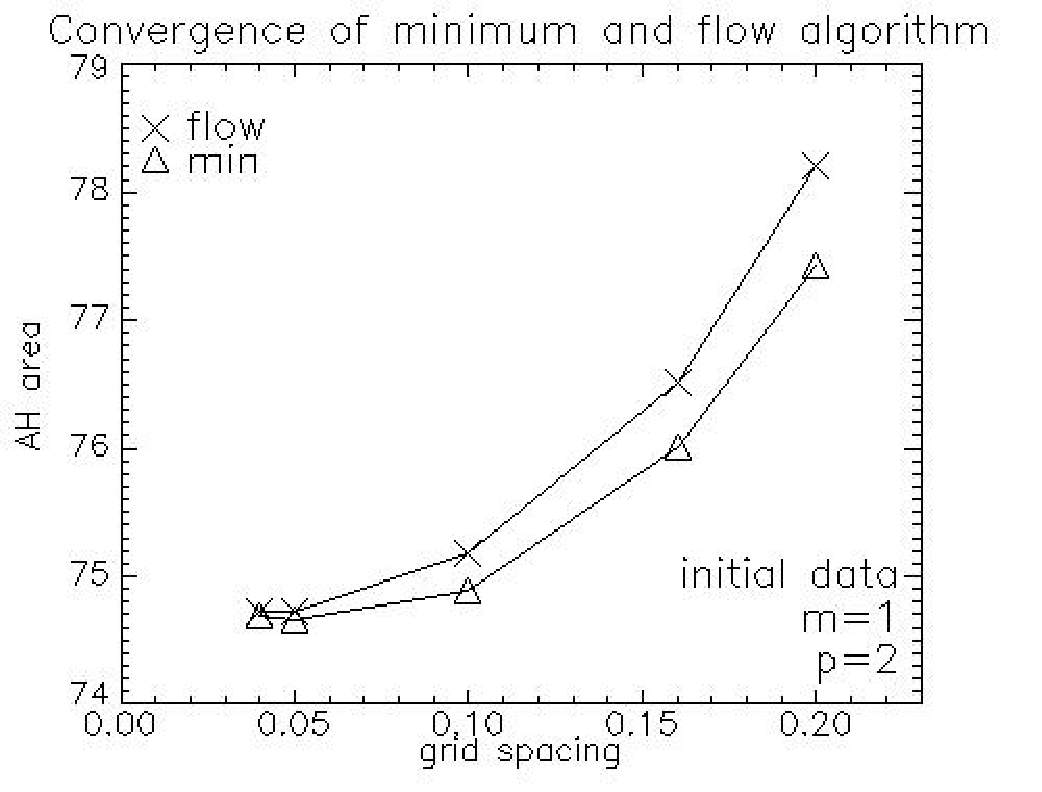
\includegraphics[angle=0,width=8cm]{p2_areacomp}
\end{center}
\caption{Convergence of the horizon area for $P_{z}=2M$}
\label{CactusEistein_AHFinder_p2_conv}
\end{figure}

Further, not only the area converges but also the shape of the horizon.
For both the minimization and the flow algorithm the horizon converges to
the same shape, as can be seen from the coefficients fo the expansion.
The order of convergence for the coefficients is between 1.4 and 1.7.

By using the parameters ahf\_xc, ahf\_yc, ahf\_zc it can also be shown that
the finder also locates horizons which are not centered. This works in
general as long as the surface can be expanded in spherical harmonics
around this point, but the error increases with the off-centering.

The parameter ahf\_r0 can be used e.g. when dealing with two black holes.
If one searches for separate horizons one can center the finder on one of
the locations of the holes and use an initial radius ahf\_r0 smaller than
the coordinate distance of the holes. With this parameter settings the
single horizon can be found faster. But also a setup with an initial
sphere of maximum radius should work at least for the flow algorithm.
This has been checked with puncture data for two holes with vanishing
linear and angular momentum for each hole (equivalent to Brill-Lindquist
data) and is shown in Figure~\ref{CactusEinstein_AHFinder_p2_conv}. 
Here for a coordinate distance of the holes of 1.6M the separated
horizons for the holes are found but no common horizon. For a coordinate
distance of 1.5M a common horizon is found and also single ones, which
are inner surfaces in this case. This coincides with other work where the
critical coordinate distance for a single horizon is between 1.53M and
1.56M (gr-qc/9809004).

\begin{figure}[ht]
\begin{center}
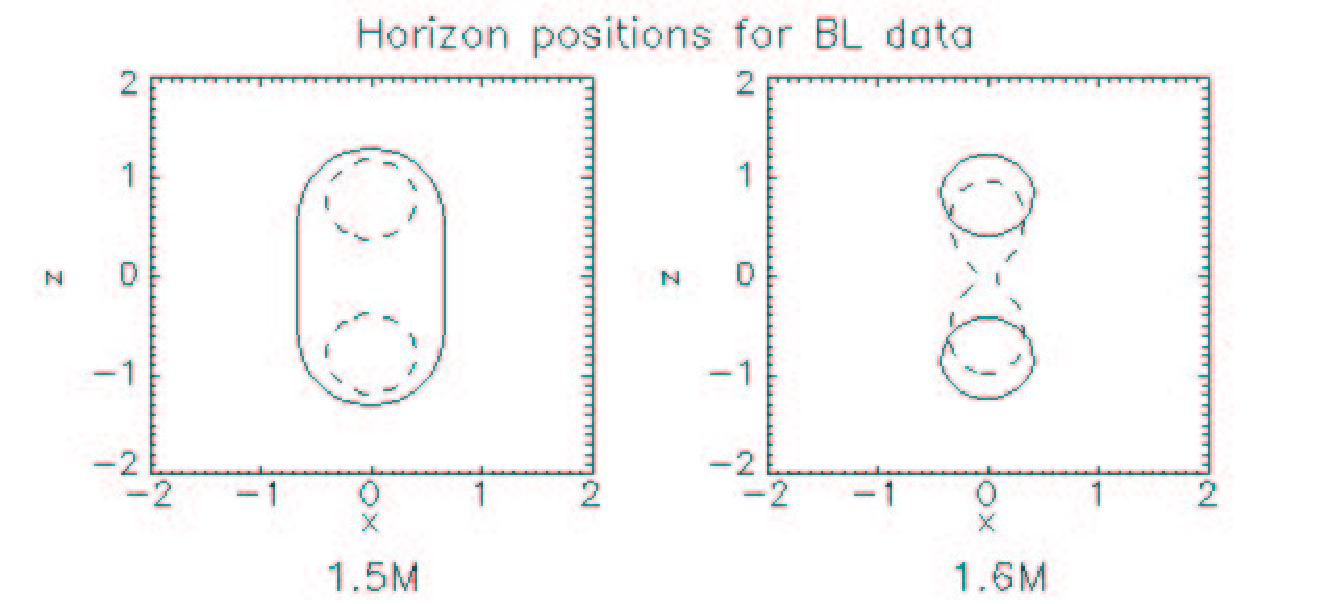
\includegraphics[angle=0,width=10cm]{hori_bl}
\end{center}
\caption{Horizon positions for BL data}
\label{CactusEinstein_AHFinder_p2_conv}
\end{figure}

The dashed lines show inner trapped surfaces in the left figure and the
surface where the algorithm stopped without finding a horizon in the
right figure.

Also the Misner case was checked. Here for $\mu$ = 1.35 a common horizon is
found. For $\mu$ = 1.37 separated horizons are found. From the literature we
know that (e.g. gr-qc/9809004) the critical value of $\mu$ is 1.36. This is
confirmed by the horizon finder.

The information of when a horizon was found can be seen in the
cactus-logfile. There will be output from the thorn even if no horizon
was found.

\begin{thebibliography}{9}

\end{thebibliography}

% Do not delete next line
% END CACTUS THORNGUIDE

\end{document}
